\documentclass[]{ctexbook}
\usepackage{lmodern}
\usepackage{amssymb,amsmath}
\usepackage{ifxetex,ifluatex}
\usepackage{fixltx2e} % provides \textsubscript
\ifnum 0\ifxetex 1\fi\ifluatex 1\fi=0 % if pdftex
  \usepackage[T1]{fontenc}
  \usepackage[utf8]{inputenc}
\else % if luatex or xelatex
  \ifxetex
    \usepackage{xltxtra,xunicode}
  \else
    \usepackage{fontspec}
  \fi
  \defaultfontfeatures{Ligatures=TeX,Scale=MatchLowercase}
\fi
% use upquote if available, for straight quotes in verbatim environments
\IfFileExists{upquote.sty}{\usepackage{upquote}}{}
% use microtype if available
\IfFileExists{microtype.sty}{%
\usepackage{microtype}
\UseMicrotypeSet[protrusion]{basicmath} % disable protrusion for tt fonts
}{}
\usepackage[a4paper,tmargin=2.5cm,bmargin=2.5cm,lmargin=3.5cm,rmargin=2.5cm]{geometry}
\usepackage[unicode=true]{hyperref}
\PassOptionsToPackage{usenames,dvipsnames}{color} % color is loaded by hyperref
\hypersetup{
            pdftitle={实验研究的设计及分析},
            pdfauthor={杨志宏},
            colorlinks=true,
            linkcolor=Maroon,
            citecolor=Blue,
            urlcolor=Blue,
            breaklinks=true}
\urlstyle{same}  % don't use monospace font for urls
\usepackage{natbib}
\bibliographystyle{GBT7714-2005}
\usepackage{color}
\usepackage{fancyvrb}
\newcommand{\VerbBar}{|}
\newcommand{\VERB}{\Verb[commandchars=\\\{\}]}
\DefineVerbatimEnvironment{Highlighting}{Verbatim}{commandchars=\\\{\}}
% Add ',fontsize=\small' for more characters per line
\usepackage{framed}
\definecolor{shadecolor}{RGB}{248,248,248}
\newenvironment{Shaded}{\begin{snugshade}}{\end{snugshade}}
\newcommand{\AlertTok}[1]{\textcolor[rgb]{0.94,0.16,0.16}{#1}}
\newcommand{\AnnotationTok}[1]{\textcolor[rgb]{0.56,0.35,0.01}{\textbf{\textit{#1}}}}
\newcommand{\AttributeTok}[1]{\textcolor[rgb]{0.77,0.63,0.00}{#1}}
\newcommand{\BaseNTok}[1]{\textcolor[rgb]{0.00,0.00,0.81}{#1}}
\newcommand{\BuiltInTok}[1]{#1}
\newcommand{\CharTok}[1]{\textcolor[rgb]{0.31,0.60,0.02}{#1}}
\newcommand{\CommentTok}[1]{\textcolor[rgb]{0.56,0.35,0.01}{\textit{#1}}}
\newcommand{\CommentVarTok}[1]{\textcolor[rgb]{0.56,0.35,0.01}{\textbf{\textit{#1}}}}
\newcommand{\ConstantTok}[1]{\textcolor[rgb]{0.00,0.00,0.00}{#1}}
\newcommand{\ControlFlowTok}[1]{\textcolor[rgb]{0.13,0.29,0.53}{\textbf{#1}}}
\newcommand{\DataTypeTok}[1]{\textcolor[rgb]{0.13,0.29,0.53}{#1}}
\newcommand{\DecValTok}[1]{\textcolor[rgb]{0.00,0.00,0.81}{#1}}
\newcommand{\DocumentationTok}[1]{\textcolor[rgb]{0.56,0.35,0.01}{\textbf{\textit{#1}}}}
\newcommand{\ErrorTok}[1]{\textcolor[rgb]{0.64,0.00,0.00}{\textbf{#1}}}
\newcommand{\ExtensionTok}[1]{#1}
\newcommand{\FloatTok}[1]{\textcolor[rgb]{0.00,0.00,0.81}{#1}}
\newcommand{\FunctionTok}[1]{\textcolor[rgb]{0.00,0.00,0.00}{#1}}
\newcommand{\ImportTok}[1]{#1}
\newcommand{\InformationTok}[1]{\textcolor[rgb]{0.56,0.35,0.01}{\textbf{\textit{#1}}}}
\newcommand{\KeywordTok}[1]{\textcolor[rgb]{0.13,0.29,0.53}{\textbf{#1}}}
\newcommand{\NormalTok}[1]{#1}
\newcommand{\OperatorTok}[1]{\textcolor[rgb]{0.81,0.36,0.00}{\textbf{#1}}}
\newcommand{\OtherTok}[1]{\textcolor[rgb]{0.56,0.35,0.01}{#1}}
\newcommand{\PreprocessorTok}[1]{\textcolor[rgb]{0.56,0.35,0.01}{\textit{#1}}}
\newcommand{\RegionMarkerTok}[1]{#1}
\newcommand{\SpecialCharTok}[1]{\textcolor[rgb]{0.00,0.00,0.00}{#1}}
\newcommand{\SpecialStringTok}[1]{\textcolor[rgb]{0.31,0.60,0.02}{#1}}
\newcommand{\StringTok}[1]{\textcolor[rgb]{0.31,0.60,0.02}{#1}}
\newcommand{\VariableTok}[1]{\textcolor[rgb]{0.00,0.00,0.00}{#1}}
\newcommand{\VerbatimStringTok}[1]{\textcolor[rgb]{0.31,0.60,0.02}{#1}}
\newcommand{\WarningTok}[1]{\textcolor[rgb]{0.56,0.35,0.01}{\textbf{\textit{#1}}}}
\usepackage{longtable,booktabs}
% Fix footnotes in tables (requires footnote package)
\IfFileExists{footnote.sty}{\usepackage{footnote}\makesavenoteenv{long table}}{}
\IfFileExists{parskip.sty}{%
\usepackage{parskip}
}{% else
\setlength{\parindent}{0pt}
\setlength{\parskip}{6pt plus 2pt minus 1pt}
}
\setlength{\emergencystretch}{3em}  % prevent overfull lines
\providecommand{\tightlist}{%
  \setlength{\itemsep}{0pt}\setlength{\parskip}{0pt}}
\setcounter{secnumdepth}{5}
% Redefines (sub)paragraphs to behave more like sections
\ifx\paragraph\undefined\else
\let\oldparagraph\paragraph
\renewcommand{\paragraph}[1]{\oldparagraph{#1}\mbox{}}
\fi
\ifx\subparagraph\undefined\else
\let\oldsubparagraph\subparagraph
\renewcommand{\subparagraph}[1]{\oldsubparagraph{#1}\mbox{}}
\fi

% set default figure placement to htbp
\makeatletter
\def\fps@figure{htbp}
\makeatother

\usepackage{booktabs}
\usepackage{longtable}

\usepackage{framed,color}
\definecolor{shadecolor}{RGB}{248,248,248}

\renewcommand{\textfraction}{0.05}
\renewcommand{\topfraction}{0.8}
\renewcommand{\bottomfraction}{0.8}
\renewcommand{\floatpagefraction}{0.75}

\let\oldhref\href
\renewcommand{\href}[2]{#2\footnote{\url{#1}}}

\makeatletter
\newenvironment{kframe}{%
\medskip{}
\setlength{\fboxsep}{.8em}
 \def\at@end@of@kframe{}%
 \ifinner\ifhmode%
  \def\at@end@of@kframe{\end{minipage}}%
  \begin{minipage}{\columnwidth}%
 \fi\fi%
 \def\FrameCommand##1{\hskip\@totalleftmargin \hskip-\fboxsep
 \colorbox{shadecolor}{##1}\hskip-\fboxsep
     % There is no \\@totalrightmargin, so:
     \hskip-\linewidth \hskip-\@totalleftmargin \hskip\columnwidth}%
 \MakeFramed {\advance\hsize-\width
   \@totalleftmargin\z@ \linewidth\hsize
   \@setminipage}}%
 {\par\unskip\endMakeFramed%
 \at@end@of@kframe}
\makeatother

\makeatletter
\@ifundefined{Shaded}{
}{\renewenvironment{Shaded}{\begin{kframe}}{\end{kframe}}}
\@ifpackageloaded{fancyvrb}{%
  % https://github.com/CTeX-org/ctex-kit/issues/331
  \RecustomVerbatimEnvironment{Highlighting}{Verbatim}{commandchars=\\\{\},formatcom=\xeCJKVerbAddon}%
}{}
\makeatother

\usepackage{makeidx}
\makeindex

\urlstyle{tt}

\usepackage{amsthm}
\makeatletter
\def\thm@space@setup{%
  \thm@preskip=8pt plus 2pt minus 4pt
  \thm@postskip=\thm@preskip
}
\makeatother

\frontmatter

\title{实验研究的设计及分析}
\author{杨志宏}
\date{2019-12-01}

\let\BeginKnitrBlock\begin \let\EndKnitrBlock\end
\begin{document}
\maketitle


\thispagestyle{empty}

\begin{center}
献给……

呃,爱谁谁吧
\end{center}

\setlength{\abovedisplayskip}{-5pt}
\setlength{\abovedisplayshortskip}{-5pt}

{
\setcounter{tocdepth}{2}
\tableofcontents
}
\listoftables
\listoffigures
\hypertarget{ux524dux8a00}{%
\chapter*{前言}\label{ux524dux8a00}}


在这本小书中,我将介绍控制实验的研究设计和数据分析。多因素实验设计是当前研究发展的趋势,它可在一定程度上克服早期实验室和现场研究的局限性,使实验研究更加深入,可探索更加复杂的现象,同时使研究结果更加精确、可靠。

同时,实验设计也是一本技术,它包括实验设计、统计分析和计算机数据处理三方面的知识,缺一不可。

以下是我的 R 进程信息:

\begin{Shaded}
\begin{Highlighting}[]
\KeywordTok{sessionInfo}\NormalTok{()}
\end{Highlighting}
\end{Shaded}

\begin{verbatim}
## R version 3.6.1 (2019-07-05)
## Platform: x86_64-apple-darwin15.6.0 (64-bit)
## Running under: macOS Catalina 10.15
## 
## Matrix products: default
## BLAS:   /Library/Frameworks/R.framework/Versions/3.6/Resources/lib/libRblas.0.dylib
## LAPACK: /Library/Frameworks/R.framework/Versions/3.6/Resources/lib/libRlapack.dylib
## 
## locale:
## [1] en_US.UTF-8/en_US.UTF-8/en_US.UTF-8/C/en_US.UTF-8/en_US.UTF-8
## 
## attached base packages:
## [1] stats     graphics  grDevices utils     datasets 
## [6] methods   base     
## 
## loaded via a namespace (and not attached):
##  [1] compiler_3.6.1  magrittr_1.5    bookdown_0.16  
##  [4] tools_3.6.1     htmltools_0.4.0 yaml_2.2.0     
##  [7] Rcpp_1.0.3      stringi_1.4.3   rmarkdown_1.18 
## [10] knitr_1.26      stringr_1.4.0   xfun_0.11      
## [13] digest_0.6.23   rlang_0.4.2     evaluate_0.14
\end{verbatim}

\BeginKnitrBlock{flushright}
杨志宏\\
于 世界之最温暖处
\EndKnitrBlock{flushright}

\mainmatter

\hypertarget{intro}{%
\chapter{实验设计概述}\label{intro}}

实验设计\index{实验设计},指的是实施实验处理的一个计划方案以及与计划方案有关的共计分析。

实验设计包括:

\begin{enumerate}
\def\labelenumi{\arabic{enumi}.}
\tightlist
\item
  建立与研究假说有关的统计假说;
\item
  确定实验中使用的实验处理(自变量)和必须控制的多余条件(无关变量);
\item
  确定实验中需要的实验单元(被试)的数量以及被试抽样的总体;
\item
  确定将实验条件分配给被试的方法;
\item
  确定实验中每个被试要记载的测量(因变量)和使用的统计分析。
\end{enumerate}

做实验研究,需要具备两方面的知识:

\begin{enumerate}
\def\labelenumi{\arabic{enumi}.}
\tightlist
\item
  有关研究课题的理论背景、研究的基本假设与预期,要保证开展的研究在特定的领域中有继承、有发展,有一定的科学价值。
\item
  有关实验研究的研究设计、统计学知识和软件操作知识。
\end{enumerate}

\hypertarget{ux5b9eux9a8cux8bbeux8ba1ux53d1ux5c55ux8d8bux52bf}{%
\section{实验设计发展趋势}\label{ux5b9eux9a8cux8bbeux8ba1ux53d1ux5c55ux8d8bux52bf}}

自17世纪经验科学发展以来,实验研究由单变量研究,向多变量研究发展。多变量研究带来的问题是,多种因素之间本来是相互关联的,要同时研究多个因素的影响,难度加大。

自20世纪初以来,实验研究有两条发展路线:

\hypertarget{ux5b9eux9a8cux5ba4ux7814ux7a76}{%
\subsection{实验室研究}\label{ux5b9eux9a8cux5ba4ux7814ux7a76}}

实验室研究\index{实验室研究}通过严密的实验控制,改变和操作极少数自变量,控制其它无关变量,以保证实验结果的可靠性,它适合研究比较单纯的问题,研究结果距离现实世界太远,研究的外部效度低。

\hypertarget{ux793eux4f1aux7814ux7a76}{%
\subsection{社会研究}\label{ux793eux4f1aux7814ux7a76}}

利用统计控制,通过合理取样大量被试,在较少或没有实验控制的情况下,探讨变量之间的关系,它的基本思想是,大样本测试可以通过统计规律保证结果的可靠性。

多因素实验设计与多元统计相结合,是近几十年的发展趋势,目的在于克服传统研究的不足,使研究情景接近现实,同时最大限度地保证结果的精度。

\hypertarget{ux591aux56e0ux7d20ux5b9eux9a8cux8bbeux8ba1ux7684ux7279ux70b9}{%
\subsection{多因素实验设计的特点}\label{ux591aux56e0ux7d20ux5b9eux9a8cux8bbeux8ba1ux7684ux7279ux70b9}}

\begin{enumerate}
\def\labelenumi{\arabic{enumi}.}
\tightlist
\item
  实验中通过实验设计方案的周密安排及相应的统计方法,尽可能地控制无关变量。
\item
  实验中尽可能容纳较多的自变量
\end{enumerate}

\hypertarget{ux5b9eux9a8cux8bbeux8ba1ux4e2dux7684ux57faux672cux6982ux5ff5}{%
\section{实验设计中的基本概念}\label{ux5b9eux9a8cux8bbeux8ba1ux4e2dux7684ux57faux672cux6982ux5ff5}}

\hypertarget{ux56e0ux7d20ux4e0eux56e0ux7d20ux5b9eux9a8cux8bbeux8ba1}{%
\subsection{因素与因素实验设计}\label{ux56e0ux7d20ux4e0eux56e0ux7d20ux5b9eux9a8cux8bbeux8ba1}}

因素\index{因素}(factor)指研究者在实验中感兴趣的一个变量,研究者通过操纵、改变它,来估计它对因变量的影响,这个变量也叫做自变量。

因素的水平\index{level}(level),是实验中所操纵的变量的每个特定的值。如灯光强度、性别、年龄。在于方差分析相结合的实验设计中,因素水平的数量不能过多。

因素设计,通常指多于一个因素的实验设计(factoral experimental design),如一个含有三个因素、每个因素有两个水平的实验设计,称为 \texttt{2X2X2} 三因素设计。

\hypertarget{ux5904ux7406ux4e0eux5904ux7406ux6c34ux5e73ux7684ux7ed3ux5408}{%
\subsection{处理与处理水平的结合}\label{ux5904ux7406ux4e0eux5904ux7406ux6c34ux5e73ux7684ux7ed3ux5408}}

处理\index{处理}(treatment)与处理水平的结合\index{处理水平的结合}(treatment combinations),是指实验中一个特定的、独特的实验条件。

\begin{quote}
被试接受A2B2实验处理,即在呈现速度为低速(A2)并且英语单词为高频单词(B2)的实验条件下,被试接受测试。
\end{quote}

\hypertarget{ux4e3bux6548ux5e94ux4e0eux4ea4ux4e92ux4f5cux7528}{%
\section{主效应与交互作用}\label{ux4e3bux6548ux5e94ux4e0eux4ea4ux4e92ux4f5cux7528}}

主效应(main effects)\index{主效应},是指一个因素的不同水平引起的变异。

\begin{figure}

{\centering 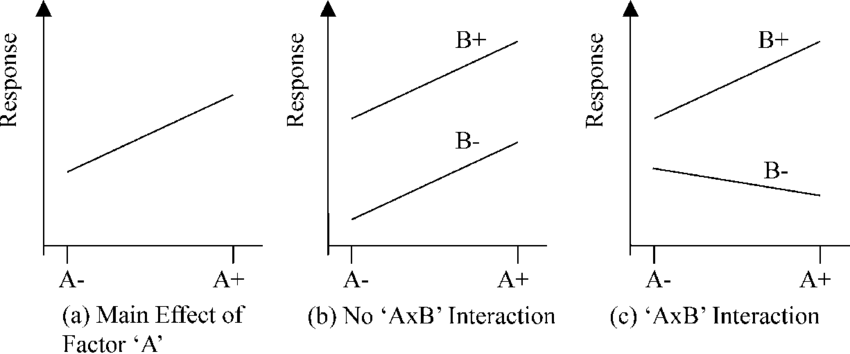
\includegraphics[width=0.9\linewidth]{images/Main-and-interaction-effects} 

}

\caption{主效应、交互作用示意图}\label{fig:maineffect}
\end{figure}

在单因素实验中,由自变量的不同水平的数据计算的方差,就是这个变量的处理效应,即主效应。

在多因素实验中,计算一个因素的主效应时,应忽略实验中其他因素的不同水平的差异。

当一个因素的水平在另一个因素的不同水平上变化趋势不一致时,我们称这两个因素之间存在交互作用(interaction)\index{交互作用}。如果变化趋势一致,表明这两个因素是相互独立的。

\hypertarget{ux7b80ux5355ux6548ux5e94}{%
\subsection{简单效应}\label{ux7b80ux5355ux6548ux5e94}}

简单效应(simple effects)\index{简单效应},指的是一个因素的水平在另一个因素的某个水平上的变异。

\begin{quote}
A 因素的两个水平在B1水平的方差,叫A在B1水平的简单效应。
\end{quote}

\hypertarget{basic}{%
\chapter{Bookdown 的基本用法}\label{basic}}

从本质上讲,bookdown 是基于 Pandoc、markdown、R、Rmarkdown、gitbook、tex、git 等等一系列开源项目上的综合性工具,这套工具大大降低了用户自己整合上述多个工具的成本,以更加高效地方式完成内容创作、发布和维护。

\hypertarget{ux4f7fux7528bookdownux521bux4f5cux7684ux6d41ux7a0b}{%
\section{使用bookdown创作的流程}\label{ux4f7fux7528bookdownux521bux4f5cux7684ux6d41ux7a0b}}

\hypertarget{ux521dux59cbux5316}{%
\subsection{初始化}\label{ux521dux59cbux5316}}

使用下载的模板或者bookdown自带的模板,创建bookdown项目。建议使用前者,因为更加适合中文内容的排版。

当然,当用户熟悉了bookdown之后,还可以在这些模板的基础上进行必要的配置,使之更加符合用户的需求。

\hypertarget{ux7f16ux8f91ux5185ux5bb9}{%
\subsection{编辑内容}\label{ux7f16ux8f91ux5185ux5bb9}}

在合适的编辑器中(建议先使用RStudio,后期熟悉后,可使用VS Code之类的功能更为复杂的通用性编辑器),按照markdown以及Rmarkdown的语法规则,进行内容的创作和编辑。

\hypertarget{ux9884ux89c8ux5185ux5bb9}{%
\subsection{预览内容}\label{ux9884ux89c8ux5185ux5bb9}}

选择 RStudio 中的``\texttt{Build\ Book}''功能,生成合适格式。还可以在控制台中键入如下命令,开启实时预览:

\begin{Shaded}
\begin{Highlighting}[]
\NormalTok{bookdown}\OperatorTok{::}\KeywordTok{serve_book}\NormalTok{()}
\end{Highlighting}
\end{Shaded}

\hypertarget{ux53d1ux5e03}{%
\subsection{发布}\label{ux53d1ux5e03}}

利用 GitHub 或 Gitee 的 page 服务,可将生成的静态页面发布到网络。

\hypertarget{bookdown-ux5bf9ux6587ux6863ux7684ux7ec4ux7ec7}{%
\section{bookdown 对文档的组织}\label{bookdown-ux5bf9ux6587ux6863ux7684ux7ec4ux7ec7}}

和一篇文章相比,一本书包含多个章节。在bookdown中,一个章节对应一个后缀名为\texttt{.Rmd}的 R Markdown 文件,每个 R Markdown 文件(除了首页)都必须以一级标题开头。例如:

\begin{Shaded}
\begin{Highlighting}[]
\FunctionTok{# bookdown 对书本文档的组织}
\end{Highlighting}
\end{Shaded}

默认情况下,bookdown 按照文件名的顺序,从前到后合并在一起,并渲染成gitbook格式或者pdf、epub或者word文件。

如果存在\texttt{index.Rmd}文件,则该文件会被渲染成\texttt{index.html}。以下划线开头的文件,会被bookdown忽略。

bookdown 还提供了自定义章节顺序的机制。在配置文件\texttt{\_bookdown.yml}中,通过\texttt{rmd\_files}字段实现,例如:

\begin{Shaded}
\begin{Highlighting}[]
\FunctionTok{rmd_files}\KeywordTok{:}\AttributeTok{ }\KeywordTok{[}\StringTok{"index.Rmd"}\KeywordTok{,}\AttributeTok{ }\StringTok{"abstract.Rmd"}\KeywordTok{,}\AttributeTok{ }\StringTok{"intro.Rmd"}\KeywordTok{]}
\end{Highlighting}
\end{Shaded}

还可以分别为不同格式指定包含的内容:

\begin{verbatim}
rmd_files:
  html: ["index.Rmd", "abstract.Rmd", "intro.Rmd"]
  latex: ["abstract.Rmd", "intro.Rmd"]
\end{verbatim}

必须要指出的是,每个章节的一级标题后,需要在后面加上标签,如:

\begin{Shaded}
\begin{Highlighting}[]
\FunctionTok{# Bookdown 的基本用法 \{#basic\}}
\end{Highlighting}
\end{Shaded}

\hypertarget{bookdown-ux8bedux6cd5}{%
\section{bookdown 语法}\label{bookdown-ux8bedux6cd5}}

首先,bookdown是基于markdown和pandoc的工具,因此,\href{https://daringfireball.net/projects/markdown/syntax}{Markdown 的原生语法}肯定是可以使用的。在此不再赘述。

其次,\href{https://pandoc.org/MANUAL.html\#pandocs-markdown}{Pandoc 在markdown语法的基础上,提供了一些增强},bookdown也是支持的。

最后,bookdown 是在 \href{https://rmarkdown.rstudio.com/index.html}{R bookdown 包}的基础上进行扩展,故而也支持 R Markdown 语法。如:

\begin{Shaded}
\begin{Highlighting}[]
\KeywordTok{dim}\NormalTok{(iris)}
\end{Highlighting}
\end{Shaded}

\begin{verbatim}
## [1] 150   5
\end{verbatim}

再如,下面的代码将列出R Markdown支持的所有语言:

\begin{Shaded}
\begin{Highlighting}[]
\KeywordTok{names}\NormalTok{(knitr}\OperatorTok{::}\NormalTok{knit_engines}\OperatorTok{$}\KeywordTok{get}\NormalTok{())}
\end{Highlighting}
\end{Shaded}

\begin{verbatim}
##  [1] "awk"         "bash"        "coffee"      "gawk"        "groovy"     
##  [6] "haskell"     "lein"        "mysql"       "node"        "octave"     
## [11] "perl"        "psql"        "Rscript"     "ruby"        "sas"        
## [16] "scala"       "sed"         "sh"          "stata"       "zsh"        
## [21] "highlight"   "Rcpp"        "tikz"        "dot"         "c"          
## [26] "fortran"     "fortran95"   "asy"         "cat"         "asis"       
## [31] "stan"        "block"       "block2"      "js"          "css"        
## [36] "sql"         "go"          "python"      "julia"       "sass"       
## [41] "scss"        "theorem"     "lemma"       "corollary"   "proposition"
## [46] "conjecture"  "definition"  "example"     "exercise"    "proof"      
## [51] "remark"      "solution"
\end{verbatim}

\hypertarget{howtodo}{%
\chapter{常用功能的实现}\label{howtodo}}

\hypertarget{ux5982ux4f55ux63d2ux5165ux53c2ux8003ux6587ux732e}{%
\section{如何插入参考文献}\label{ux5982ux4f55ux63d2ux5165ux53c2ux8003ux6587ux732e}}

\begin{enumerate}
\def\labelenumi{\arabic{enumi}.}
\item
  插入参考文献时,需要创建.bib格式的参考文献数据库。
\item
  在合适的地方插入引用\citep{xie2015},语法\citep{毛向樱2018}如下:

\begin{verbatim}
引用[@xie2015]
\end{verbatim}
\item
  单独创建一个显示全部参考文献的.Rmd文件,内容如下:

\begin{verbatim}
\end{verbatim}
\end{enumerate}

按照上述步骤,将在章节末尾和全书末尾生成参考文献。

\hypertarget{ux5982ux4f55ux5c06ux53c2ux8003ux6587ux732eux683cux5f0fux8c03ux6574ux4e3aux56fdux6807ux683cux5f0f}{%
\section{如何将参考文献格式调整为国标格式}\label{ux5982ux4f55ux5c06ux53c2ux8003ux6587ux732eux683cux5f0fux8c03ux6574ux4e3aux56fdux6807ux683cux5f0f}}

在首页文件\texttt{index.Rmd}中,用户可以通过\texttt{biblio-style}指定参考文献的格式,例如:

\begin{Shaded}
\begin{Highlighting}[]
\PreprocessorTok{---}
\FunctionTok{bibliography}\KeywordTok{:}\AttributeTok{ }\KeywordTok{[}\StringTok{"one.bib"}\KeywordTok{,}\AttributeTok{ }\StringTok{"another.bib"}\KeywordTok{,}\AttributeTok{ }\StringTok{"yet-another.bib"}\KeywordTok{]}
\FunctionTok{biblio-style}\KeywordTok{:}\AttributeTok{ }\StringTok{"GBT7714-2005"}
\FunctionTok{link-citations}\KeywordTok{:}\AttributeTok{ }\CharTok{true}
\PreprocessorTok{---}
\end{Highlighting}
\end{Shaded}

与此同时,还需要将上述文件复制到项目目录中,不过上述设定,仅对PDF和word输出时起作用,对于gitbook格式,则没有效果。

\bibliography{book.bib,packages.bib}

\backmatter
\printindex

\end{document}
